\documentclass{article}%
\usepackage[T1]{fontenc}%
\usepackage[utf8]{inputenc}%
\usepackage{lmodern}%
\usepackage{textcomp}%
\usepackage{lastpage}%
\usepackage[head=40pt,margin=0.5in,bottom=0.6in]{geometry}%
\usepackage{graphicx}%
%
\title{\textbf{Docentes, personal obrero y administrativo de Fe y Alegría protestaron para exigir salarios justos}}%
\author{JOSÉ SILVA}%
\date{20/11/2018}%
%
\begin{document}%
\normalsize%
\maketitle%
\textbf{URL: }%
http://www.eluniversal.com/politica/26236/docentes{-}y{-}personal{-}obrero{-}de{-}fe{-}y{-}alegria{-}protestaron{-}para{-}exigir{-}salarios{-}justos\newline%
%
\textbf{Periodico: }%
EU, %
ID: %
26236, %
Seccion: %
politica\newline%
%
\textbf{Palabras Claves: }%
NO\_TIENE\newline%
%
\textbf{Derecho: }%
2.2%
, Otros Derechos: %
2.3%
, Sub Derechos: %
2.2.1, 2.3.4%
\newline%
%
\textbf{EP: }%
SI\newline%
\newline%
%
\textbf{\textit{Las manifestaciones se produjeron en diversos colegios de Caracas, así como en los estados Zulia, Carabobo, Aragua, Miranda y Sucre. Los profesores expresaron que su sueldo no les alcanza}}%
\newline%
\newline%
%
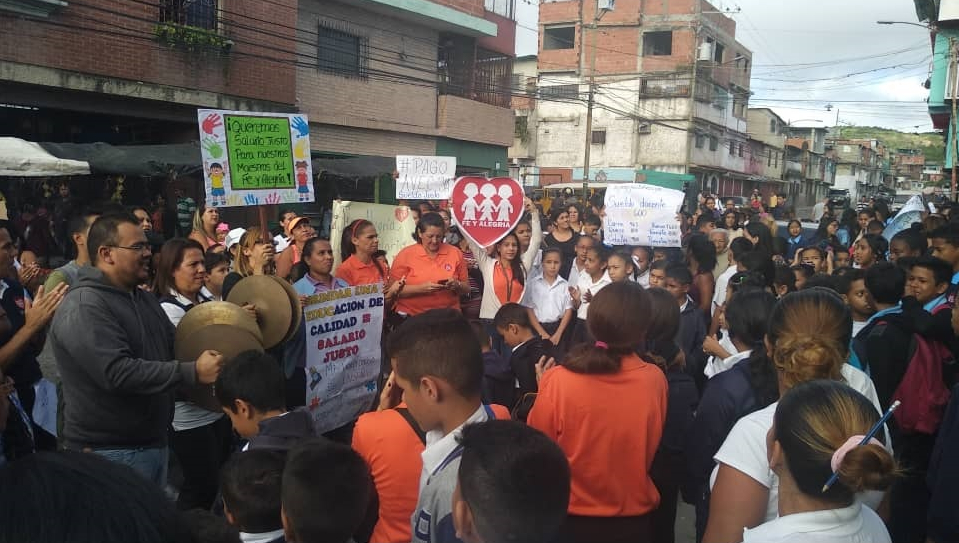
\includegraphics[width=300px]{110.jpg}%
\newline%
%
Caracas.{-} Profesores y personal que labora en los colegios Fe y Alegría de Venezuela protestaron la mañana de este martes en la capital y diversos estados del país para exigir mejoras salariales.%
\newline%
%
"A nuestro personal docente, administrativo y obrero no le alcanza el salario mensual, mucho menos el pago de forma semanal" reseñó la institución a través de su cuenta en la red social Twitter.%
\newline%
%
Al oeste de la capital, en La Vega, se registró una manifestación de docentes del Fe y Alegría ubicado en Las Casitas; mientras que al otro extremo, en Puente Baloa, Petare, hicieron lo propio.%
\newline%
%
Los educadores señalaron que continúan ofreciendo educación de calidad, pero que el salario que devengan no les alcanza para cubrir las necesidades básicas.%
\newline%
%
Diversos Fe y Alegría de estados como Zulia, Carabobo, Aragua, Miranda y Sucre también se sumaron a la manifestación.%
\newline%
%
Venezuela, sumida en una grave crisis económica, política y social, registró 1.418 protestas en octubre mayormente por derechos salariales, según un informe del Observatorio Venezolano de Conflictividad Social (OVCS).%
\newline%
%
Luego de la entrada en vigencia del salario mínimo en 1.800 bolívares soberanos (Bs.S), trabajadores de diversos entes de la administración pública han manifestado para exigir que se respeten los contratos colectivos.%
\newline%
%
\end{document}